\documentclass[slidestop]{beamer}
\usepackage{beamerthemesplit}
\usepackage{graphics}
\usepackage{pstricks}

\graphicspath{{./}}

\title{The Libre-SOC Hybrid 3D CPU}
\author{Luke Kenneth Casson Leighton}


\begin{document}

\frame{
   \begin{center}
    \huge{The Libre-SOC Hybrid 3D CPU}\\
    \vspace{32pt}
    \Large{Augmenting the OpenPOWER ISA}\\
    \Large{to provide 3D and Video instructions}\\
    \Large{(properly and officially)}\\
    \vspace{24pt}
    \Large{[proposed for] OpenPOWER Summit 2020}\\
    \vspace{16pt}
    \large{\today}
  \end{center}
}


\frame{\frametitle{Why another SoC?}

\vspace{15pt}

 \begin{itemize}
   \item Intel Management Engine, QA issues, Spectre\vspace{15pt}
   \item Endless proprietary drivers \\
   		 (affects product development cost)\vspace{15pt}
   \item Opportunity to drastically simplify driver development\\
	     and engage in "long-tail" markets\vspace{15pt}
   \item Because for 30 years I Always Wanted To Design A CPU\vspace{10pt}
  \end{itemize}
}


\frame{\frametitle{Why OpenPOWER? (but first: Evaluation Criteria)}

\vspace{15pt}

 \begin{itemize}
   \item Good ecosystem essential\\
   		 linux kernel, u-boot, compilers, OSes,\\
   		 Reference Implementation(s)\vspace{12pt}
   \item Supportive Foundation and Members\\
   		 need to be able to submit ISA augmentations\\
   		 (for proper peer review)\vspace{12pt}
   \item No NDAs, full transparency must be acceptable\\
	     due to being funded under NLnet's PET Programme\vspace{12pt}
  \end{itemize}
}

\frame{\frametitle{Why OpenPOWER?}


 \begin{itemize}
   \item RISC-V: closed secretive mailing lists, closed secretive\\
   		 ISA Working Groups, no acceptance of transparency\\
   		 requirements, not well-established enough
   \item MIPS Open Initiative website was offline
   \item ARM and x86 are proprietary (x86 too complex)
   \item OpenRISC 1200 not enough adoption
   \item Nyuzi GPU too specialist (not a general-purpose ISA)
   \item MIAOW GPU is not a GPU (it's an AMD Vector Engine)
   \item "rolling your own" out of the question (20+ man-years)
   \item OpenPOWER: established for decades, excellent Foundation,\\
   	     Microwatt as Reference, approachable and friendly.
  \end{itemize}
}



\frame{\frametitle{Simple SBC-style SoC}

\begin{center}
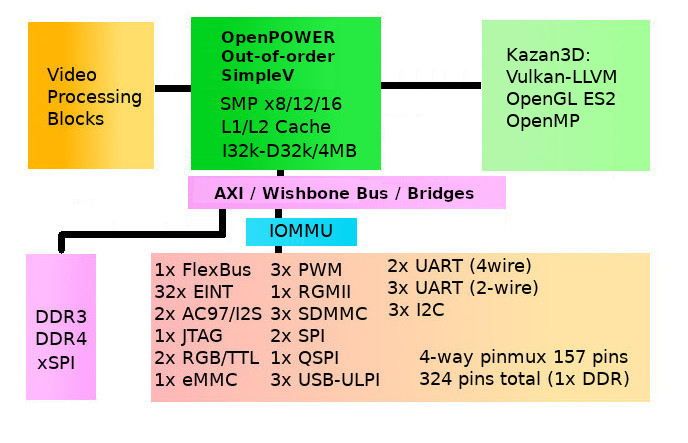
\includegraphics[width=0.9\textwidth]{shakti_libre_soc.jpg}
\end{center}

}



\frame{\frametitle{Summary}

 \begin{itemize}
   \item Actually about parallelism, not Vectors (or SIMD) per se\\
         and NOT about adding new ALU/logic/functionality.
  \end{itemize}
}


\frame{
  \begin{center}
    {\Huge The end\vspace{15pt}\\
		   Thank you\vspace{15pt}\\
		   Questions?\vspace{15pt}
	}
  \end{center}
  
  \begin{itemize}
	\item Discussion: Libre-SOC-dev mailing list
	\item Freenode IRC \#libre-soc
	\item http://libre-soc.org/
  \end{itemize}
}


\end{document}
